% Created by tikzDevice version 0.12.3.1 on 2022-05-01 18:40:29
% !TEX encoding = UTF-8 Unicode
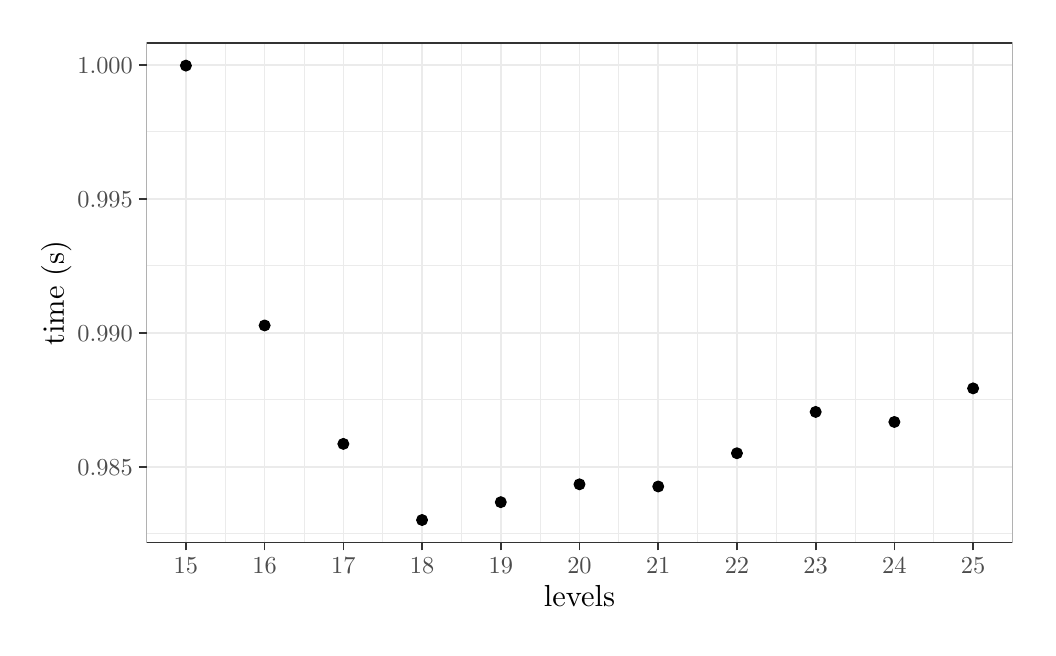
\begin{tikzpicture}[x=1pt,y=1pt]
\definecolor{fillColor}{RGB}{255,255,255}
\path[use as bounding box,fill=fillColor,fill opacity=0.00] (0,0) rectangle (361.35,216.81);
\begin{scope}
\path[clip] (  0.00,  0.00) rectangle (361.35,216.81);
\definecolor{drawColor}{RGB}{255,255,255}
\definecolor{fillColor}{RGB}{255,255,255}

\path[draw=drawColor,line width= 0.6pt,line join=round,line cap=round,fill=fillColor] (  0.00,  0.00) rectangle (361.35,216.81);
\end{scope}
\begin{scope}
\path[clip] ( 42.95, 30.69) rectangle (355.85,211.31);
\definecolor{fillColor}{RGB}{255,255,255}

\path[fill=fillColor] ( 42.95, 30.69) rectangle (355.85,211.31);
\definecolor{drawColor}{gray}{0.92}

\path[draw=drawColor,line width= 0.3pt,line join=round] ( 42.95, 33.91) --
	(355.85, 33.91);

\path[draw=drawColor,line width= 0.3pt,line join=round] ( 42.95, 82.33) --
	(355.85, 82.33);

\path[draw=drawColor,line width= 0.3pt,line join=round] ( 42.95,130.75) --
	(355.85,130.75);

\path[draw=drawColor,line width= 0.3pt,line join=round] ( 42.95,179.17) --
	(355.85,179.17);

\path[draw=drawColor,line width= 0.3pt,line join=round] ( 42.95, 30.69) --
	( 42.95,211.31);

\path[draw=drawColor,line width= 0.3pt,line join=round] ( 71.40, 30.69) --
	( 71.40,211.31);

\path[draw=drawColor,line width= 0.3pt,line join=round] ( 99.84, 30.69) --
	( 99.84,211.31);

\path[draw=drawColor,line width= 0.3pt,line join=round] (128.29, 30.69) --
	(128.29,211.31);

\path[draw=drawColor,line width= 0.3pt,line join=round] (156.73, 30.69) --
	(156.73,211.31);

\path[draw=drawColor,line width= 0.3pt,line join=round] (185.18, 30.69) --
	(185.18,211.31);

\path[draw=drawColor,line width= 0.3pt,line join=round] (213.62, 30.69) --
	(213.62,211.31);

\path[draw=drawColor,line width= 0.3pt,line join=round] (242.07, 30.69) --
	(242.07,211.31);

\path[draw=drawColor,line width= 0.3pt,line join=round] (270.51, 30.69) --
	(270.51,211.31);

\path[draw=drawColor,line width= 0.3pt,line join=round] (298.96, 30.69) --
	(298.96,211.31);

\path[draw=drawColor,line width= 0.3pt,line join=round] (327.40, 30.69) --
	(327.40,211.31);

\path[draw=drawColor,line width= 0.3pt,line join=round] (355.85, 30.69) --
	(355.85,211.31);

\path[draw=drawColor,line width= 0.6pt,line join=round] ( 42.95, 58.12) --
	(355.85, 58.12);

\path[draw=drawColor,line width= 0.6pt,line join=round] ( 42.95,106.54) --
	(355.85,106.54);

\path[draw=drawColor,line width= 0.6pt,line join=round] ( 42.95,154.96) --
	(355.85,154.96);

\path[draw=drawColor,line width= 0.6pt,line join=round] ( 42.95,203.38) --
	(355.85,203.38);

\path[draw=drawColor,line width= 0.6pt,line join=round] ( 57.18, 30.69) --
	( 57.18,211.31);

\path[draw=drawColor,line width= 0.6pt,line join=round] ( 85.62, 30.69) --
	( 85.62,211.31);

\path[draw=drawColor,line width= 0.6pt,line join=round] (114.07, 30.69) --
	(114.07,211.31);

\path[draw=drawColor,line width= 0.6pt,line join=round] (142.51, 30.69) --
	(142.51,211.31);

\path[draw=drawColor,line width= 0.6pt,line join=round] (170.96, 30.69) --
	(170.96,211.31);

\path[draw=drawColor,line width= 0.6pt,line join=round] (199.40, 30.69) --
	(199.40,211.31);

\path[draw=drawColor,line width= 0.6pt,line join=round] (227.85, 30.69) --
	(227.85,211.31);

\path[draw=drawColor,line width= 0.6pt,line join=round] (256.29, 30.69) --
	(256.29,211.31);

\path[draw=drawColor,line width= 0.6pt,line join=round] (284.74, 30.69) --
	(284.74,211.31);

\path[draw=drawColor,line width= 0.6pt,line join=round] (313.18, 30.69) --
	(313.18,211.31);

\path[draw=drawColor,line width= 0.6pt,line join=round] (341.63, 30.69) --
	(341.63,211.31);
\definecolor{drawColor}{RGB}{0,0,0}
\definecolor{fillColor}{RGB}{0,0,0}

\path[draw=drawColor,line width= 0.4pt,line join=round,line cap=round,fill=fillColor] ( 57.18,203.10) circle (  1.96);

\path[draw=drawColor,line width= 0.4pt,line join=round,line cap=round,fill=fillColor] ( 85.62,109.21) circle (  1.96);

\path[draw=drawColor,line width= 0.4pt,line join=round,line cap=round,fill=fillColor] (114.07, 66.41) circle (  1.96);

\path[draw=drawColor,line width= 0.4pt,line join=round,line cap=round,fill=fillColor] (142.51, 38.90) circle (  1.96);

\path[draw=drawColor,line width= 0.4pt,line join=round,line cap=round,fill=fillColor] (170.96, 45.35) circle (  1.96);

\path[draw=drawColor,line width= 0.4pt,line join=round,line cap=round,fill=fillColor] (199.40, 51.80) circle (  1.96);

\path[draw=drawColor,line width= 0.4pt,line join=round,line cap=round,fill=fillColor] (227.85, 51.02) circle (  1.96);

\path[draw=drawColor,line width= 0.4pt,line join=round,line cap=round,fill=fillColor] (256.29, 63.03) circle (  1.96);

\path[draw=drawColor,line width= 0.4pt,line join=round,line cap=round,fill=fillColor] (284.74, 77.96) circle (  1.96);

\path[draw=drawColor,line width= 0.4pt,line join=round,line cap=round,fill=fillColor] (313.18, 74.33) circle (  1.96);

\path[draw=drawColor,line width= 0.4pt,line join=round,line cap=round,fill=fillColor] (341.63, 86.47) circle (  1.96);
\definecolor{drawColor}{gray}{0.20}

\path[draw=drawColor,line width= 0.6pt,line join=round,line cap=round] ( 42.95, 30.69) rectangle (355.85,211.31);
\end{scope}
\begin{scope}
\path[clip] (  0.00,  0.00) rectangle (361.35,216.81);
\definecolor{drawColor}{gray}{0.30}

\node[text=drawColor,anchor=base east,inner sep=0pt, outer sep=0pt, scale=  0.88] at ( 38.00, 55.09) {0.985};

\node[text=drawColor,anchor=base east,inner sep=0pt, outer sep=0pt, scale=  0.88] at ( 38.00,103.51) {0.990};

\node[text=drawColor,anchor=base east,inner sep=0pt, outer sep=0pt, scale=  0.88] at ( 38.00,151.93) {0.995};

\node[text=drawColor,anchor=base east,inner sep=0pt, outer sep=0pt, scale=  0.88] at ( 38.00,200.35) {1.000};
\end{scope}
\begin{scope}
\path[clip] (  0.00,  0.00) rectangle (361.35,216.81);
\definecolor{drawColor}{gray}{0.20}

\path[draw=drawColor,line width= 0.6pt,line join=round] ( 40.20, 58.12) --
	( 42.95, 58.12);

\path[draw=drawColor,line width= 0.6pt,line join=round] ( 40.20,106.54) --
	( 42.95,106.54);

\path[draw=drawColor,line width= 0.6pt,line join=round] ( 40.20,154.96) --
	( 42.95,154.96);

\path[draw=drawColor,line width= 0.6pt,line join=round] ( 40.20,203.38) --
	( 42.95,203.38);
\end{scope}
\begin{scope}
\path[clip] (  0.00,  0.00) rectangle (361.35,216.81);
\definecolor{drawColor}{gray}{0.20}

\path[draw=drawColor,line width= 0.6pt,line join=round] ( 57.18, 27.94) --
	( 57.18, 30.69);

\path[draw=drawColor,line width= 0.6pt,line join=round] ( 85.62, 27.94) --
	( 85.62, 30.69);

\path[draw=drawColor,line width= 0.6pt,line join=round] (114.07, 27.94) --
	(114.07, 30.69);

\path[draw=drawColor,line width= 0.6pt,line join=round] (142.51, 27.94) --
	(142.51, 30.69);

\path[draw=drawColor,line width= 0.6pt,line join=round] (170.96, 27.94) --
	(170.96, 30.69);

\path[draw=drawColor,line width= 0.6pt,line join=round] (199.40, 27.94) --
	(199.40, 30.69);

\path[draw=drawColor,line width= 0.6pt,line join=round] (227.85, 27.94) --
	(227.85, 30.69);

\path[draw=drawColor,line width= 0.6pt,line join=round] (256.29, 27.94) --
	(256.29, 30.69);

\path[draw=drawColor,line width= 0.6pt,line join=round] (284.74, 27.94) --
	(284.74, 30.69);

\path[draw=drawColor,line width= 0.6pt,line join=round] (313.18, 27.94) --
	(313.18, 30.69);

\path[draw=drawColor,line width= 0.6pt,line join=round] (341.63, 27.94) --
	(341.63, 30.69);
\end{scope}
\begin{scope}
\path[clip] (  0.00,  0.00) rectangle (361.35,216.81);
\definecolor{drawColor}{gray}{0.30}

\node[text=drawColor,anchor=base,inner sep=0pt, outer sep=0pt, scale=  0.88] at ( 57.18, 19.68) {15};

\node[text=drawColor,anchor=base,inner sep=0pt, outer sep=0pt, scale=  0.88] at ( 85.62, 19.68) {16};

\node[text=drawColor,anchor=base,inner sep=0pt, outer sep=0pt, scale=  0.88] at (114.07, 19.68) {17};

\node[text=drawColor,anchor=base,inner sep=0pt, outer sep=0pt, scale=  0.88] at (142.51, 19.68) {18};

\node[text=drawColor,anchor=base,inner sep=0pt, outer sep=0pt, scale=  0.88] at (170.96, 19.68) {19};

\node[text=drawColor,anchor=base,inner sep=0pt, outer sep=0pt, scale=  0.88] at (199.40, 19.68) {20};

\node[text=drawColor,anchor=base,inner sep=0pt, outer sep=0pt, scale=  0.88] at (227.85, 19.68) {21};

\node[text=drawColor,anchor=base,inner sep=0pt, outer sep=0pt, scale=  0.88] at (256.29, 19.68) {22};

\node[text=drawColor,anchor=base,inner sep=0pt, outer sep=0pt, scale=  0.88] at (284.74, 19.68) {23};

\node[text=drawColor,anchor=base,inner sep=0pt, outer sep=0pt, scale=  0.88] at (313.18, 19.68) {24};

\node[text=drawColor,anchor=base,inner sep=0pt, outer sep=0pt, scale=  0.88] at (341.63, 19.68) {25};
\end{scope}
\begin{scope}
\path[clip] (  0.00,  0.00) rectangle (361.35,216.81);
\definecolor{drawColor}{RGB}{0,0,0}

\node[text=drawColor,anchor=base,inner sep=0pt, outer sep=0pt, scale=  1.10] at (199.40,  7.64) {levels};
\end{scope}
\begin{scope}
\path[clip] (  0.00,  0.00) rectangle (361.35,216.81);
\definecolor{drawColor}{RGB}{0,0,0}

\node[text=drawColor,rotate= 90.00,anchor=base,inner sep=0pt, outer sep=0pt, scale=  1.10] at ( 13.08,121.00) {time (s)};
\end{scope}
\end{tikzpicture}
